\documentclass[a4paper,12pt,oneside,openright,final]{memoir}

\usepackage[table]{xcolor}
\usepackage{graphicx}
\usepackage[portuguese,ruled,vlined]{algorithm2e}
\SetKwFor{Para}{para}{fa�a}{fim para}
\SetKwRepeat{Do}{do}{while}
\usepackage{algorithmic}
\usepackage{adjustbox}
\usepackage{setspace}
\usepackage{url}
\usepackage{amsmath}
\usepackage{amsthm}
\usepackage{mathrsfs}
\usepackage{mathptmx}
\usepackage{amssymb}
\usepackage{bbm}
\usepackage{verbatim}
\usepackage{calc}
\usepackage{multirow}
\usepackage{pagina}
\usepackage{nomes}
\usepackage{pbox}
\usepackage{subcaption}
\usepackage{epstopdf}
\usepackage{cite}
\usepackage[brazil]{babel}
\usepackage[utf8,latin1]{inputenc}
\usepackage{graphicx}
\usepackage{caption}
%\usepackage{abntex2cite}
%\usepackage{abntex2abrev}
%\usepackage{hyperref}
\usepackage{enumerate}
%\usepackage[brazilian]{babel}
\usepackage[T1,T2A]{fontenc}
\usepackage{amssymb}
%\usepackage[portuguese]{babel}
\usepackage[
    a4paper,
    portuguese,
    bookmarks=true,
    bookmarksnumbered=true,
    linktocpage,
    ]{hyperref}
\usepackage{memhfixc}
\usepackage{listings}
\usepackage{marvosym}
\usepackage{pgf}
\usepackage{float}
\usepackage{indentfirst}
\usepackage{verbatim}
%\usepackage{tikz}
%\usetikzlibrary{arrows,automata,positioning,trees,shapes}
\usepackage{mdframed}
\usepackage[T1]{fontenc}
\usepackage{tabularx}
\usepackage{rotating, graphicx}
\linespread{1.5}

\usepackage{pdfpages}

\setlrmarginsandblock{3cm}{2cm}{*}
\setulmarginsandblock{3cm}{3cm}{*}
\setheaderspaces{2cm}{*}{*}

\checkandfixthelayout

\makeheadrule{myheadings}{\textwidth}{\normalrulethickness}
\makeoddhead{myheadings}{\textsc{\leftmark}}{}{\thepage}

\copypagestyle{contents}{myheadings}
\makeoddhead{contents}{\textsc{\contentsname}}{}{\thepage}

\copypagestyle{bibliography}{myheadings}
\makeoddhead{bibliography}{\textsc{\bibname}}{}{\thepage}

\makeatletter

\def\mychaptermark#1{%
	\markboth{%
	\ifnum \c@secnumdepth >\m@ne
		\if@mainmatter
			\thechapter. \ %
		\fi
	\fi
	#1}{}}%

\def\mysectionmark#1{%
\markright{%
	\ifnum \c@secnumdepth > \z@
		\thesection. \ %
	\fi
	#1}}%

\makeatother

\maxsecnumdepth{subsubsection}

\newcommand{\tableformat}{\small\centering}
\newcommand{\figureformat}{\centering}

\renewcommand{\labelenumi}{\alph{enumi})}
\renewcommand{\labelenumii}{\arabic{enumii}.}

\setcounter{tocdepth}{2} %-- ajusta produndidade do indice

\let\Chapter\chapter
\def\chapter{\addtocontents{lol}{\protect\addvspace{10pt}}\Chapter}

\renewcommand{\lstlistingname}{Algoritmo}
\renewcommand{\lstlistlistingname}{Lista de Algoritmos}

\lstset{
  numbers=left,
  stepnumber=1,
  firstnumber=1,
  numberstyle=\tiny,
  extendedchars=true,
  breaklines=true,
  frame=tb,
  basicstyle=\footnotesize,
  stringstyle=\ttfamily,
  showstringspaces=false,
  captionpos=b,
  breakautoindent=truem
  language=C,
  numbersep=5pt,
  tabsize=2,
  morekeywords={assert,enquanto,se,fim,entao,senao,retorne,faca,assume,Passo,for,int,long, unsigned,while}
}

\makeatletter
\renewcommand\l@lstlisting[2]{\@dottedtocline{1}{0cm}{0.95cm}{#1}{#2}}
\makeatother

\newcolumntype{P}[1]{>{\centering\arraybackslash}p{#1}}

\usepackage{parskip}
\setlength{\parindent}{35pt}

\begin{document}

\newcommand{\limit}[3] {\ensuremath{\lim_{#1 \rightarrow #2} #3}}
\newtheorem{definition}{Defini��o}[chapter]
\newtheorem{lemma}{Lema}[chapter]
\newtheorem{theorem}{Teorema}[chapter]

\newtheorem{fact}{Fact}[chapter]
\newtheorem{example}{Exemple}[chapter]

%---------------------------------------------------------------------
% -- Titulo e Descricao %---------------------------------------------------------------------

\newcommand{\tittese}{%
	\textsf{\bfseries\Large Localiza��o de Rob�s M�veis Baseada em Odometria e Vis�o Computacional\\
	\vspace{0.8ex}
        }}

\newcommand{\descrtese}{%
\hspace{\stretch{1}}\parbox{0.51\textwidth}{%
Monografia apresentada � Coordena��o do Curso
de Engenharia El�trica - Eletr�nica da Universidade Federal
do Amazonas, como parte dos requisitos necess�rios
� obten��o do t�tulo de Engenheiro Eletricista.
}}

%---------------------------------------------------------------------
% -- Capa %---------------------------------------------------------------------

\frontmatter
\pagestyle{empty}

\begin{center}


\includegraphics[bb=0 0 646 638,height=2.5cm]{figuras/ufam.png}

\textsf{\large%
Universidade Federal do Amazonas\\
Faculdade de Tecnologia\\
Engenharia El�trica - Eletr�nica}

\vspace*{4cm}
\vspace*{\stretch{1}}

\tittese

\vspace*{4cm}
\vspace*{\stretch{1}}

{\large Alexandre de Assis Ribeiro}

\vspace*{3cm}
\vspace*{\stretch{1}}

Manaus -- Amazonas

Dezembro de 2018

\end{center}

%---------------------------------------------------------------------
% -- Contracapa %---------------------------------------------------------------------

\begin{center}

{\large Alexandre de Assis Ribeiro}

\vspace*{4cm}
\vspace*{\stretch{2}}

\tittese

\vspace*{2cm}
\vspace*{\stretch{1}}

\descrtese

\vspace*{2cm}
\vspace*{\stretch{1}}

Orientador: Prof. Dr. Jo�o Edgar Chaves Filho \\

\end{center}

%---------------------------------------------------------------------
% -- Banca Examinadora %---------------------------------------------------------------------
%
%\begin{center}
%
%{\large Rodrigo Farias Ara�jo}
%
%\vspace*{3cm}
%%\vspace*{\stretch{2}}
%
%\tittese
%
%\vspace*{2cm}
%%\vspace*{\stretch{1}}
%
%Banca Examinadora
%\vspace{2em}
%
%Prof. Dr. Jo�o Edgar Chaves Filho\\
%Departamento de Eletricidade - UFAM
%\vspace{2em}
%
%Prof. Dr-Ing Vicente Ferreira de Lucena Junior \\
%Departamento de Eletr�nica e Computa��o - UFAM
%\vspace{2em}
%
%Prof.� Dra. Fab�ola Guerra Nakamura\\
%Instituto de Computa��o - UFAM
%\vspace{2em}
%
%\vspace*{\stretch{0.5}}
%
%Manaus -- Amazonas
%
%Mar�o de 2017
%
%\end{center}
%
%\cleardoublepage
%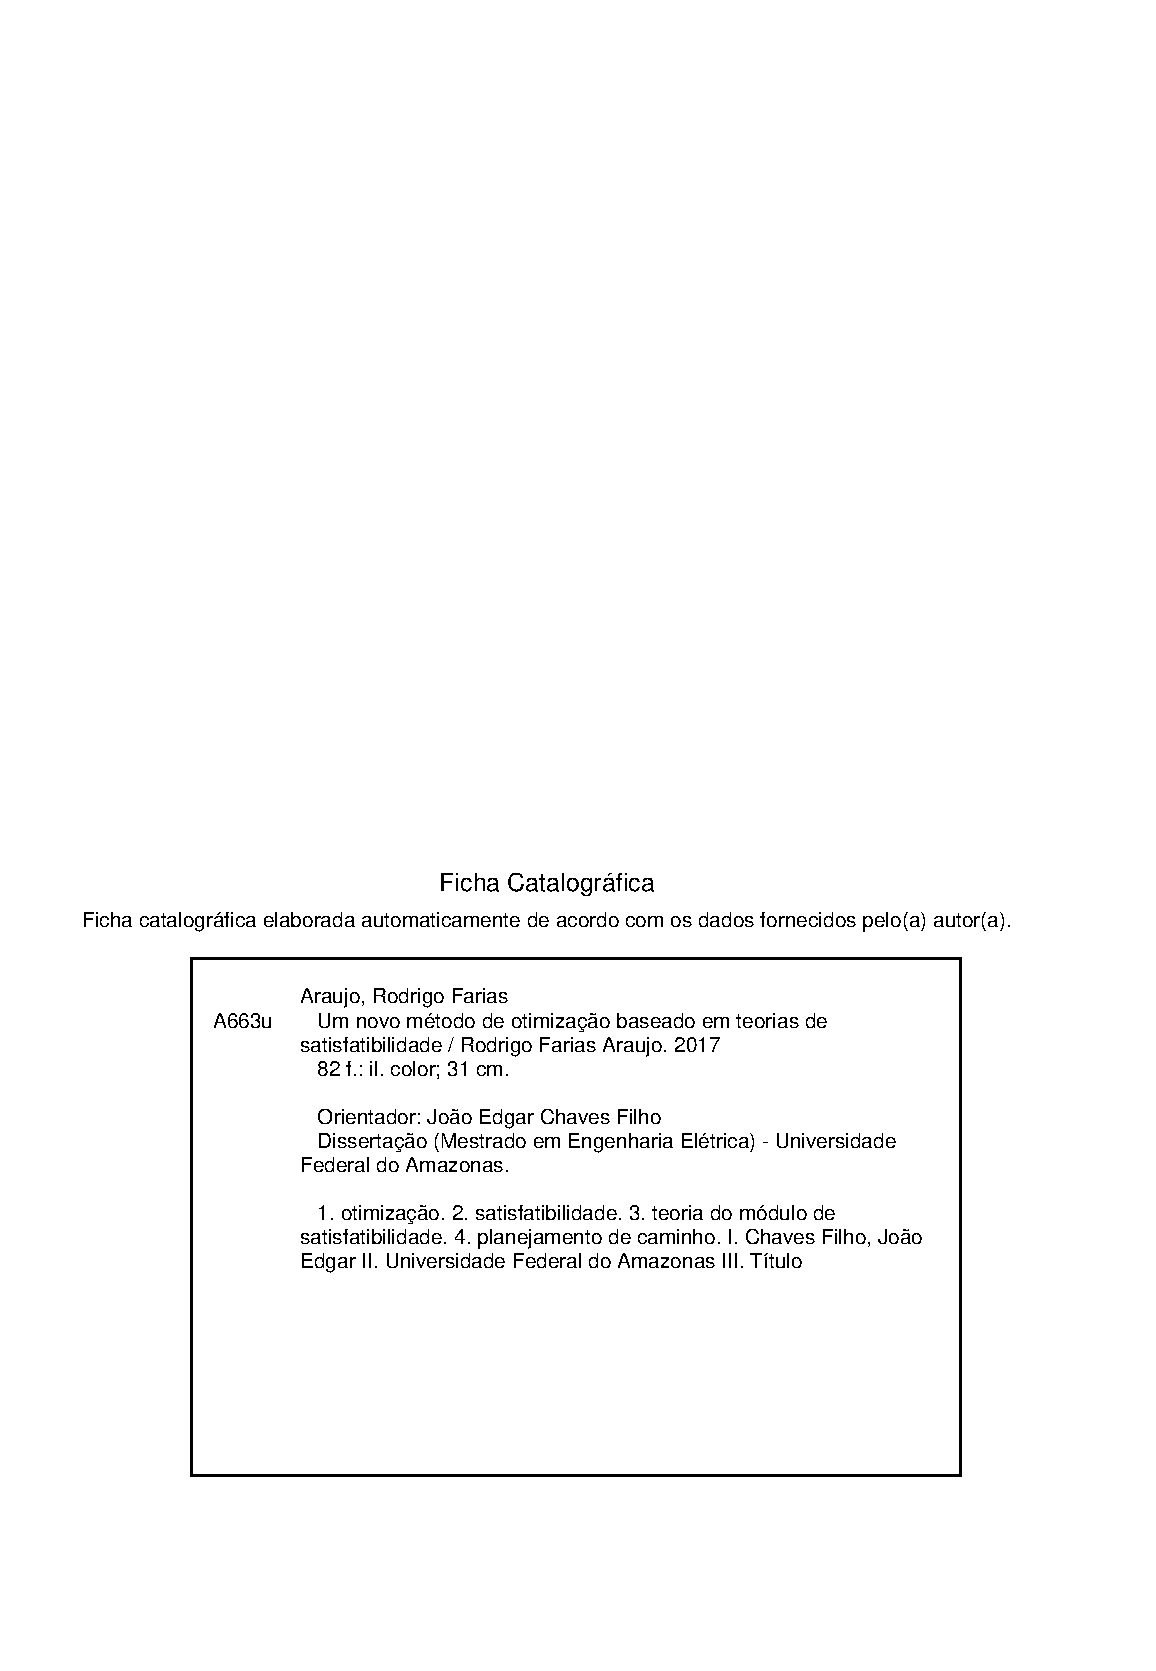
\includepdf[pages=1]{0_capa/ficha_catalografica.pdf}
%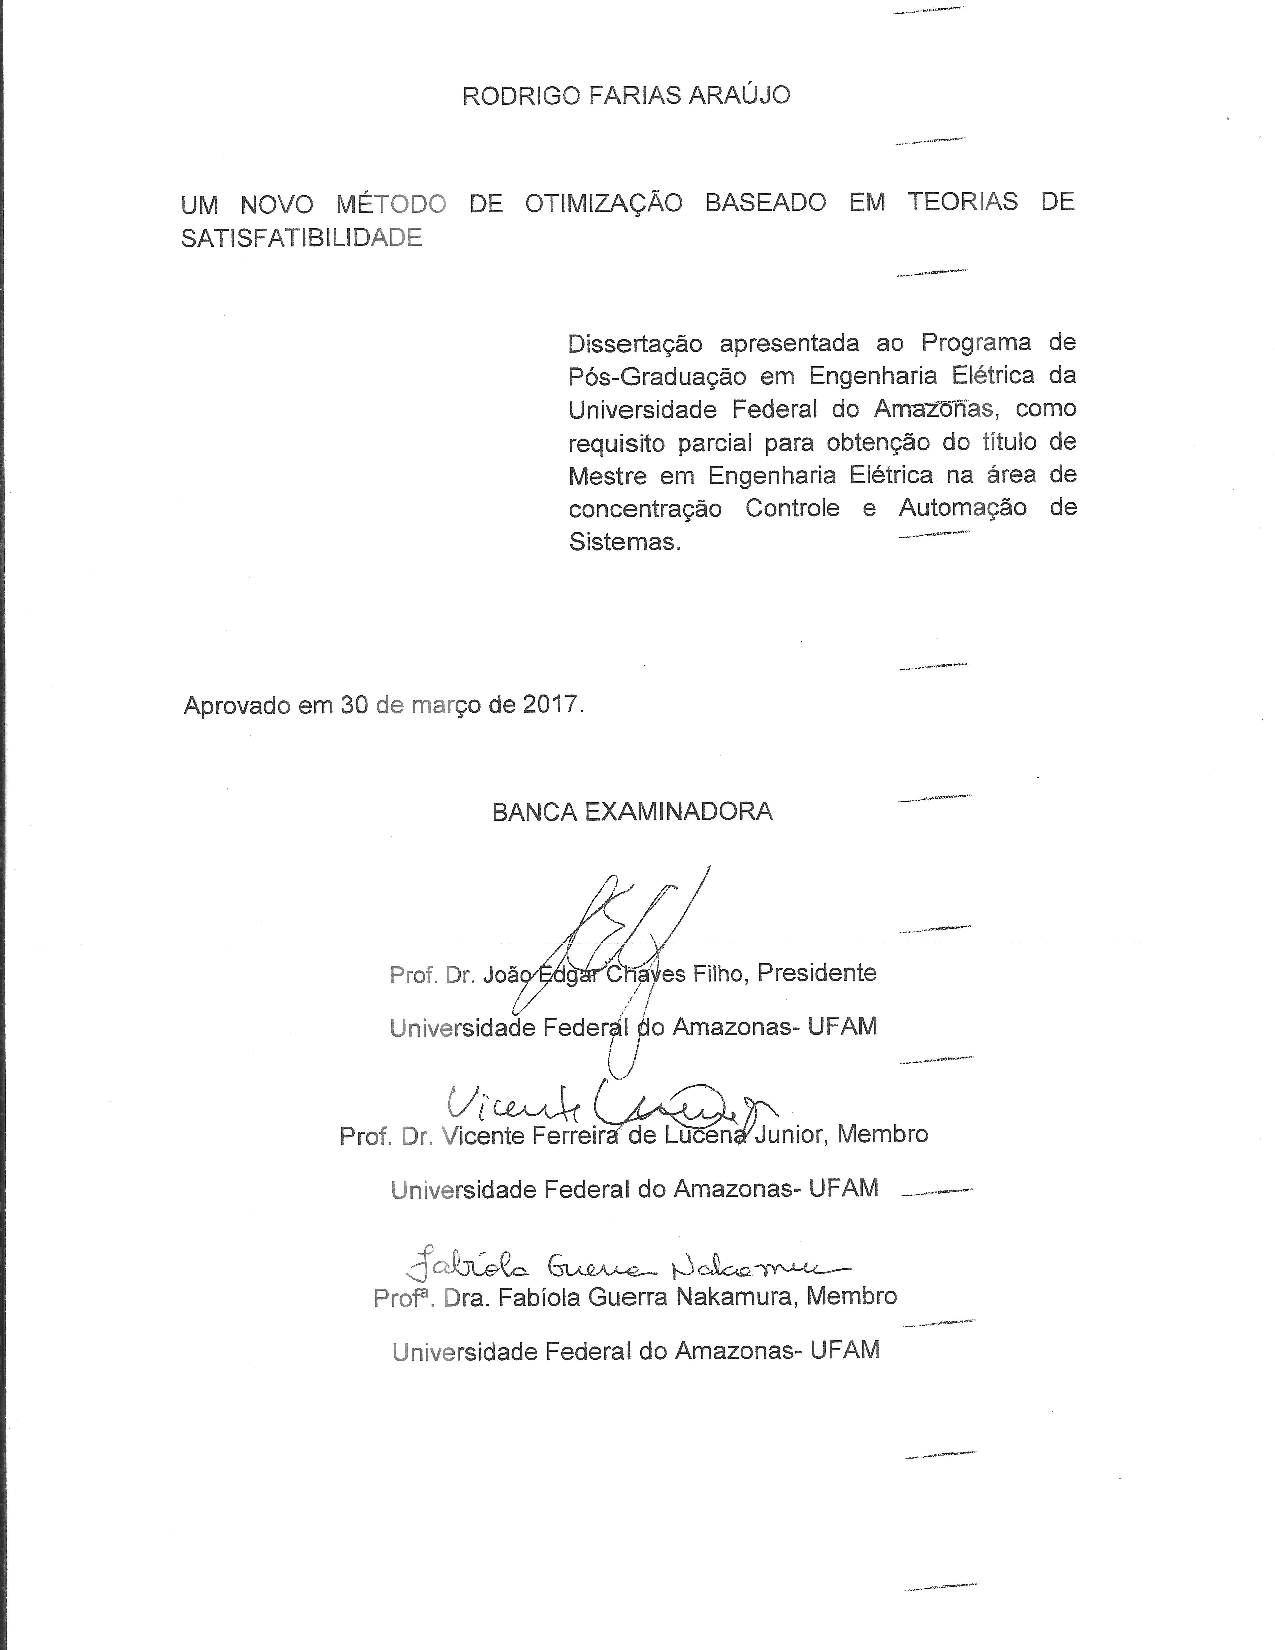
\includepdf[pages=1]{0_capa/banca.pdf}
%\cleardoublepage

%--------------------------------------------------------------
% -- Dedicat�ria %--------------------------------------------------------------

\vspace*{\stretch{2}}
%
\begin{flushright}
\textit{� minha m�e.}\hspace{1cm}
\end{flushright}

\vspace*{\stretch{1}}

\cleardoublepage

%--------------------------------------------------------------
% -- Agradecimentos %--------------------------------------------------------------

\chapter*{Agradecimentos}

\thispagestyle{empty}

%{\doublespacing

%\setlength{\parindent}{0cm}

Agrade�o primeiramente � minha m�e e meu pai, Raimunda e Reginaldo, por me apoiarem e guiarem desde sempre. Agrade�o a minha namorada Adria por sempre me incentivar e apoiar durante o mestrado.

Agrade�o aos amigos e colegas da UEA e UFAM que acumulei ao longo da gradua��o e do mestrado, em especial ao Iury Bessa pela ajuda durante o mestrado.

Agrade�o ao Prof. Jo�o Edgar por todos os ensinamentos, conselhos, orienta��es e suporte ao longo do mestrado. Ao Prof. Lucas Cordeiro pelo suporte e conselhos.

Agrade�o finalmente a toda a equipe de professores PPGEE/UFAM que ajudaram a sedimentar essa forma��o.

\vspace*{3cm}
\cleardoublepage

%----------------------------------------------------------------
% -- Ep�grafe %-----------------------------------------------------------------

%{\singlespacing
\vspace*{1cm}
\vspace*{\stretch{1}}

\hspace{\stretch{1}}\parbox{0.5\textwidth}{
\begin{flushright}
\emph{One can achieve a great success when we stay true to ourselves.}
\end{flushright}
}
\vspace{2em}

\hspace{\stretch{1}}{\emph{Friedrich Nietzche}}

\vspace*{\stretch{1}}
%-------------------------------------------------------------------
% -- Resumo %-------------------------------------------------------------------
\chapter*{Resumo}
\thispagestyle{empty}
Este trabalho apresenta um sistema de monitoramento e controle remoto de baixo custo para condicionadores de ar, que
utiliza conceitos de Internet das Coisas. A principal ferramenta utilizada foi o microcontrolador ESP8266, que atrav�s do protocolo MQTT recebe e retorna requisi��es de um aplicativo \textit{mobile} pela internet. Foram utilizados um sensor de presen�a, para
alertar o consumo desnecess�rio de energia, dispositivos de acionamento el�trico para acionar a carga e foi desenvolvido um circuito medidor de energia el�trica para informar o consumo do condicionador de ar. Al�m disso, foi utilizado o protocolo \textit{Network Time Protocol} para sincronizar o
rel�gio do microprocessador, desta maneira foi poss�vel ligar e desligar o condicionador de ar conforme hor�rio escolhido no aplicativo. Por fim � apresentado um comparativo experimental da medi��o do consumo de energia el�trica entre o prot�tipo desenvolvido e um medidor de energia j� difundido no mercado, de modo a validar o sistema para implanta��o.

\vspace*{\stretch{1}} %texto se adapta para ocupar toda a p�gina

\noindent \textsf{Palavras-chave:} Internet das coisas, condicionador de ar, ESP8266, MQTT, controle remoto.

\cleardoublepage

%-------------------------------------------------------------------
% -- Abstract %-------------------------------------------------------------------
\chapter*{Abstract}
\thispagestyle{empty}

This work presents a remote monitoring and control system for low cost air conditioners, which
uses Internet of Things concepts. The main tool used was the ESP8266 microcontroller, which through the MQTT protocol receives and returns requests from a mobile application. A presence sensor was used to
alerting unnecessary energy consumption, electric drive devices to power the load and an energy meter was developed to inform the consumption of the air conditioner. The Network Time Protocol was used to synchronize the
microprocessor clock, this way it was possible to turn on and off the air conditioner according to the chosen time in the application. For programming the microcontroller, the C ++ programming language was used along with the Arduino software,
which contains all the functions needed to develop the system.

\vspace*{\stretch{1}} %texto se adapta para ocupar toda a pagina

\noindent \textsf{Keywords:} Internet of Things, Air Conditioner, ESP8266, MQTT, Remote Control.

\cleardoublepage


%------------------------------------------------------------------
% �ndices
%------------------------------------------------------------------

\pagestyle{contents}
\pagenumbering{roman}

\tableofcontents*  % gera o �ndice (sum�rio)
\cleardoublepage

%\phantomsection
%\addcontentsline{toc}{chapter}{\listfigurename}
%\listoffigures*    % gera a lista de figuras
%\cleardoublepage

%\phantomsection
%\addcontentsline{toc}{chapter}{\listtablename}
%\listoftables*     % gera a lista de tabelas
%\cleardoublepage

%\newcommand{\algorithmname}{Algoritmo}
%\newcommand{\listalgorithmname}{Lista de Algoritmos} %\newlistof{listofalgorithms}{loa}{\listalgorithmname}

%\phantomsection
%\addcontentsline{toc}{chapter}{\listalgorithmname}
%\listofalgorithms*
%\cleardoublepage

\chapter{Abrevia��es}
\label{appendix:abreviacao}

\noindent 
\textbf{PCB}	-	\textit{Placa de circuito impresso - do ingl�s \textbf{P}rinted \textbf{C}ircut \textbf{B}oard} \\
\textbf{USB}	-	\textit{Barramento universal serial - do ingl�s \textbf{U}niversal \textbf{S}erial \textbf{B}us} \\
\textbf{I2C}	-	\textit{Circuito inter-integrado - do ingl�s \textbf{I}nter-\textbf{I}ntegrated \textbf{C}ircuit} \\
\textbf{UART}	-	\textit{Receptor-transmissor universal ass�ncrono - do ingl�s \textbf{U}niversal \textbf{A}ssyncronous \textbf{R}eceiver-\textbf{T}ransmitter} \\
\textbf{MQTT}	-	\textit{Protocolo de mensagens entre m�quinas - do ingl�s \textbf{M}essage \textbf{Q}ueuing \textbf{T}elemetry \textbf{T}ransport} \\
\textbf{LED}	-	\textit{Diodo emissor de luz - do ingl�s \textbf{L}ight-\textbf{E}mitting \textbf{D}iode}\\


\mainmatter
\pagestyle{myheadings}

\let\chaptermark=\mychaptermark
\let\sectionmark=\mysectionmark

\setcounter{secnumdepth}{3}	% ajusta profundidade da contagem de s�ries

%%%%%%%%%%%%%%%%%%%%%%%%%%%%%%%%%%%%%%%%%%%%%%
\chapter{Introdu��o}
\label{chapter:introducao}
%%%%%%%%%%%%%%%%%%%%%%%%%%%%%%%%%%%%%%%%%%%%%%

%%%%%%%%%%%%%%%%%%%%%%%%%%%%%%%%%%%%%%%%%%%%%%%
\section{Objetivo Geral}
%%%%%%%%%%%%%%%%%%%%%%%%%%%%%%%%%%%%%%%%%%%%%%%

%%%%%%%%%%%%%%%%%%%%%%%%%%%%%%%%%%%%%%%%%%%%%%%
\section{Objetivos Espec�ficos}
%%%%%%%%%%%%%%%%%%%%%%%%%%%%%%%%%%%%%%%%%%%%%%%

%%%%%%%%%%%%%%%%%%%%%%%%%%%%%%%%%%%%%%%%%%%%%%%
\section{Planejamento do Projeto}
%%%%%%%%%%%%%%%%%%%%%%%%%%%%%%%%%%%%%%%%%%%%%%%


%%%%%%%%%%%%%%%%%%%%%%%%%%%%%%%%%%%%%%%%%%%%%%
\chapter{Fundamenta��o Te�rica}
\label{chapter:fundamentacao_teorica}
%%%%%%%%%%%%%%%%%%%%%%%%%%%%%%%%%%%%%%%%%%%%%%
Este cap�tulo apresenta os fundamentos te�ricos utilizados para o desenvolvimento deste trabalho. Primeiramente, a se��o \ref{sec:iot_mqtt} explanar� a Internet das Coisas (IoT) e um dos protocolos mais utilizados por esta tecnologia, o \textit{Message Queuing Telemetry Transport} (MQTT), que � um dos protocolos mais utilizados quando se trata de comunica��o neste tipo de rede. Em seguida, na se��o \ref{sec:dispositivos_acionamento_eletrico}, ser�o abordados os dispositivos utilizados quando se trata de acionamentos el�tricos, dando enfoque aos respons�veis pelo acionamento de cargas do tipo resistiva e indutiva. Por final ser� abordado, na se��o \ref{sec:medicao_energia_eletrica}, a medi��o de energia el�trica e os Circuitos Integrados de Gerenciamento de Energia (PMICs), enfatizando suas utiliza��es em sistemas de monitoramento da qualidade da energia el�trica.

\section{Internet das Coisas e o Protocolo MQTT}
\label{sec:iot_mqtt}
O termo Internet das Coisas (do ingl�s Internet of Things - IoT) foi utilizado a primeira vez em 1999 por Kevin Ashton durante uma apresenta��o para executivos da Procter \& Gamble (P\&G), para se referir a implementa��o de tecnologia RFID (Radio-Frequency IDentification) na cadeia de suprimentos da P\&G com o objetivo de informatizar o sistema de estoque e torn�-lo mais preciso, minimizando a atua��o humana t�o suscet�vel a falhas \cite{kevin_ashton}. Apesar de, no primeiro momento, o termo utilizado referir-se a aplica��o de uma tecnologia espec�fica, o conceito de IoT se ampliou com o passar dos anos a partir dos avan�os tecnol�gicos que tornaram a sua aplicabilidade vi�vel e cada vez mais frequente \cite{santos_etal}.

Atualmente, a defini��o de IoT pode receber abordagens variadas, a depender da �tica sob a qual est� sendo relatada. Como definido por Atzori et al em seu artigo de 2010, a IoT pode ser apresentada sob tr�s perspectivas: 1) vis�o orientada �s coisas: com enfoque para os objetos; 2) vis�o orientada � Internet: com foco para a comunica��o e as redes; 3) vis�o orientada a sem�ntica: trata da interpreta��o dos dados gerados \cite{atzori}. 

De forma geral, a IoT pode ser definida como uma extens�o da Internet, que permite dispositivos f�sicos estabelecerem comunica��o entre si ou com pessoas, atrav�s da rede mundial de computadores, possibilitando ao usu�rio adquirir e monitorar informa��es, al�m de permitir a conex�o independente entre objetos inteligentes \cite{santos_etal}.

A aplica��o da tecnologia Iot se estende aos mais diversos setores, podendo ser direcionada para interesses individuais, como no uso residencial para economia de energia, por exemplo, ou para interesses da sociedade em ocorr�ncias de maior impacto como monitoramento de cheias, informa��es sobre terremotos, dados sobre o tr�fego, monitoramento de pacientes internados, entre outros \cite{gubbi}. Dessa forma, a evolu��o da IoT constitui uma importante ferramenta no desenvolvimento de cidades inteligentes a partir do trabalho colaborativo entre diferentes sistemas em resposta �s situa��es de forma autom�tica \cite{iot_open_data}.

O progresso da IoT � de interesse tanto da ind�stria, como da academia, onde h� uma elevada expectativa sobre o uso desta tecnologia, sendo considerada a maior aposta para se apresentar como a nova revolu��o da tecnologia da informa��o \cite{kevin_ashton}. Isto se d� em raz�o do seu potencial de uso nas mais diversas �reas das atividades humanas a fim de trazer avan�os na automa��o residencial e industrial \cite{santos_etal}.

Em rela��o a estrutura, a IoT abrange a infraestrutura geral de funcionamento, incluindo software, hardware e servi�os, que � usada para sustentar essas redes de informa��es. Para realizar a identifica��o dispositivos, � poss�vel usar tecnologias de identifica��o como, por exemplo, RFID, que permitem que cada dispositivo seja identificado de forma �nica \cite{gubbi}. 

A IoT apresenta sua arquitetura que pode ser didaticamente dividida em camadas projetadas para responder �s demandas de diferentes ind�strias, empresas e sociedade. As camadas da arquitetura s�o e suas funcionalidades s�o \cite{zarghami}:

\begin{itemize}
	\setlength\itemsep{0em}
	\item Camada de Borda: camada de hardware que consiste em sistemas embarcados, etiquetas RFID, redes de sensores e todos os outros sensores em diferentes formas. Essa camada de hardware pode executar v�rias fun��es, como coleta de informa��es de um sistema ou ambiente, processamento de informa��es e apoio � comunica��o.
	\item Camada de Acesso: direcionada ao manuseio de dados e � respons�vel por publicar e assinar os servi�os fornecidos pelo objeto, pelo roteamento de mensagens e pela comunica��o entre as plataformas.
	\item Camada de Internet: respons�vel por prover a comunica��o e acesso � rede mundial de computadores.
	Camada de \textit{middleware}: atua como intermedi�ria entre as camadas de Internet e de Aplica��o, sendo capaz de agregar e filtrar os dados recebidos dos dispositivos de hardware, realizando a descoberta de informa��es e fornecendo controle de acesso aos dispositivos para aplicativos.
	\item Camada de aplica��o: tem por objetivo processar os dados coletados na camada de hardware prover servi�os espec�ficos aos usu�rios. 
\end{itemize}

Entendendo que o funcionamento da IoT baseia-se no compartilhamento de dados via Internet e que para integrar v�rios dispositivos em uma rede � necess�rio uma padroniza��o de comunica��o, o Protocolo MQTT (Message Queue Telemetry Transport) apresenta-se como uma op��o de protocolo de comunica��o de n�vel de aplica��o seguro e vi�vel \cite{iot_open_data}.

\begin{figure}[H]
	\centering
	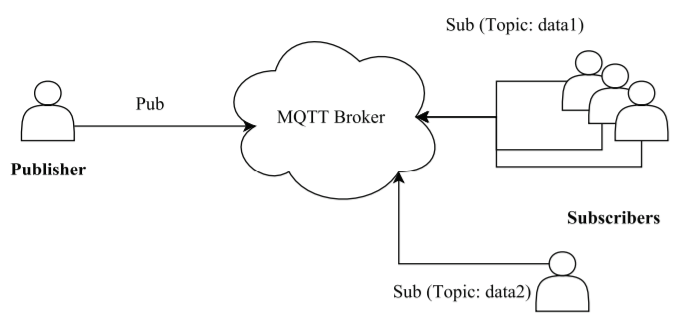
\includegraphics[width=0.7\columnwidth]{figuras/mqtt_architecture}
	\caption{Arquitetura de funcionamento no protocolo MQTT \cite{iot_open_data}.}
	\label{fig:mqtt_architecture}
\end{figure}

o Protocolo  MQTT � um protocolo de comunica��o baseado na estrat�gia de publisher/subscriber, � leve, possui pouca largura de banda, permite v�rios clientes conectados simultaneamente a um �nico servidor e garante que a mensagem seja enviada, al�m de possuir a licen�a livre de royalties o que o torna ideal para aplica��es de IoT. O MQTT � o Protocolo mais popular entre os protocolos de comunica��o devido ao seu peso e a sua capacidade de compartilhar muitos dados em tempo real. (MQTT, 2017)

O MQTT foi desenvolvido para ser usado sobre o protocolo TCP/IP (Transmition Control Protocol e Internet Protocol) e situa-se na camada de aplica��o deste Protocolo que � respons�vel por fazer a comunica��o entre os programas invocados pelos usu�rios e os protocolos de transporte. (Yuan, 2018)

\begin{figure}[H]
	\centering
	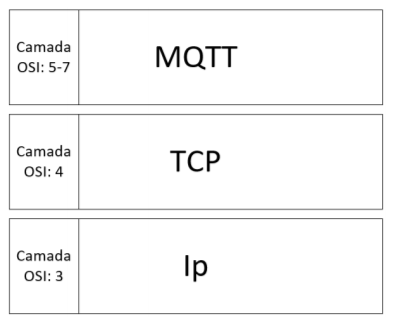
\includegraphics[width=0.5\columnwidth]{figuras/mqtt_osi}
	\caption{As camadas do protocolo MQTT \cite{tcc_sistema_de_monitoramento_residencial}.}
	\label{fig:mqtt_osi}
\end{figure}

A arquitetura do MQTT envolve tr�s componentes principais: o Publisher e o Subscriber - que podem ser denominados como Clients - e o Broker. O Publisher � o dispositivo inteligente respons�vel por se conectar ao servidor para enviar informa��es, enquanto o Subscriber � respons�vel por escolher as informa��es que ser�o recebidas. � denominado de Broker o servidor que faz a intermedia��o entre Publisher e Subscriber, ao receber e organizar as mensagens enviadas pelo Publisher e envi�-las ao Subscriber \cite{iot_open_data}.

O protocolo MQTT � orientado por mensagens em que cada mensagem � um peda�o discreto de dados. Toda mensagem � publicada em um endere�o conhecido como t�pico. Os Clients podem se inscrever em v�rios t�picos e todo cliente inscrito em um t�pico recebe todas as mensagens publicadas em tal t�pico. Como, por exemplo, em uma rede simples com tr�s Clients e um Broker, todos os tr�s Clients abrem conex�es TCP com o Broker.



\section{Dispositivos de Acionamento El�trico}
\label{sec:dispositivos_acionamento_eletrico}

Os dispositivos de acionamentos el�tricos s�o componentes usados em sistemas automatizados que recebem comandos de circuitos el�tricos, acionando as cargas, ou seja, permitindo ou n�o a passagem de corrente el�trica entre um ou mais pontos dos circuitos a serem controlados. Dentre os dispositivos de comando dispon�veis, aqueles respons�veis por realizar a fun��o de comuta��o, ou seja, respons�veis por estabelecer, interromper e, no caso de varia��o de velocidade, regular o valor de corrente absorvida por uma carga podem ser representados pelos rel�s e pelas contatoras, que s�o  componentes eletromec�nicos respons�veis por impedir ou permitir a passagem de corrente el�trica entre a fonte e a carga atrav�s de manobras (ligar e desligar), e destinam-se a ligar e desligar a carga de forma segura, ou seja, sem que haja o contato do operador no circuito de pot�ncia, onde circula a maior corrente. Apesar de os rel�s eletromagn�ticos e contatoras apresentarem fun��es semelhantes,  eles se diferem por caracter�sticas pr�prias em comportamento e aplica��o \cite{apostila_acionamentos}.

\subsection{Rel�s}
O rel� � um dispositivo el�trico respons�vel por produzir modifica��es s�bitas e predeterminadas em um ou mais circuitos el�tricos de sa�da, quando alcan�adas determinadas condi��es no circuito de entrada, que controla o dispositivo. Assim, o rel� n�o possui a fun��o de interromper o circuito principal, mas sim atuar como um sistema de manobra \cite{radiografia}. 

Os rel�s s�o compostos, de modo geral, por um eletro�m�, em forma de bobina; uma armadura met�lica, que possa ser atra�da pelo campo magn�tico criado pelo eletro�m�; uma mola e um conjunto de contatos el�tricos, que ser�o abertos, fechados ou comutados, conforme a configura��o de cada rel�. A corrente el�trica, ao percorrer a bobina, d� origem a um campo magn�tico que atrai a armadura e provoca a altera��o da posi��o dos contatos, gerando a abertura, fechamento ou comuta��o, a depender de posi��o e do tipo de rel�, fazendo o dispositivo atuar. 

Os rel�s s�o os elementos fundamentais de manobra de cargas el�tricas, pois permitem a combina��o de l�gicas no comando, bem como a separa��o dos circuitos de pot�ncia e comando. A figura \ref{fig:acionamentos_rele} representa um rel� em seu modo mais simples, composto de uma carca�a com cinco terminais. Os terminais (1) e (2) representam a bobina de excita��o, o terminal (3) representa o terminal de entrada, e os terminais (4) e (5) correspondem aos contatos normalmente fechado (NF) e normalmente aberto (NA), respectivamente. Uma caracter�stica importante dos rel�s � que n�o h� contato f�sico entre os terminais de acionamento e os de trabalho, o que permite o surgimento de dois circuitos simult�neos em um painel el�trico, sendo:

\begin{figure}[H]
	\centering
	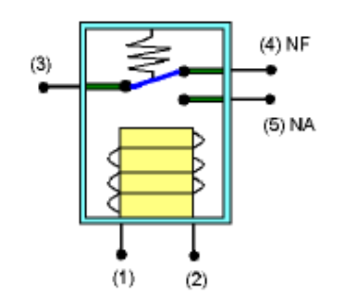
\includegraphics[width=0.4\columnwidth]{figuras/acionamentos_rele}
	\caption{Diagrama esquem�tico de um rel� \cite{acionamentos}.}
	\label{fig:acionamentos_rele}
\end{figure}

i. Circuito de comando: onde encontra-se a interface com o operador da m�quina ou dispositivo e portanto trabalha com baixas correntes (at� 10 A) e/ou baixas tens�es.
ii. Circuito de Pot�ncia: onde se encontram as cargas a serem acionadas, tais como motores, resist�ncias de aquecimento, entre outras. Neste podem circular correntes el�tricas da ordem de 10 A ou mais, e atingir tens�es de at� 760 V.


\subsection{Contatoras}

As contatoras, elementos principais de comandos eletromec�nicos, s�o dispositivos de manobra mec�nica, que permitem o controle de elevadas correntes por meio de um circuito de baixa corrente, constru�dos para uma elevada freq��ncia de opera��o.

Uma contatora consiste basicamente de um n�cleo magn�tico bipartido, em que h� uma parte m�vel e a outra fixa e uma bobina. Quando a bobina eletromagn�tica � energizada, forma-se um campo magn�tico que se concentra na parte fixa do dispositivo e atrai o n�cleo m�vel, onde est�o localizados os contatos m�veis, que, por consequ�ncia, tamb�m s�o deslocados. Quando n�o h� corrente circulando pela bobina de excita��o, a parte fixa do n�cleo � repelida por a��o de molas. Contatos el�tricos s�o distribu�dos solidariamente a parte m�vel do n�cleo, constituindo um conjunto de contatos m�veis. Mutuamente a carca�a da contatora existe um conjunto de contatos fixos. Cada jogo de contatos fixos e m�veis podem ser do tipo Normalmente aberto (NA), ou normalmente fechados (NF).

\begin{figure}[H]
	\centering
	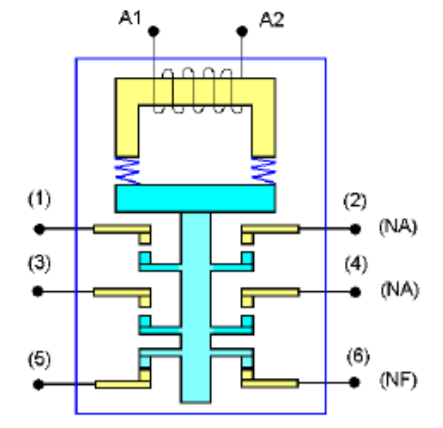
\includegraphics[width=0.4\columnwidth]{figuras/acionamentos_contatora}
	\caption{Diagrama esquem�tico de uma contatora \cite{acionamentos}.}
	\label{fig:acionamentos_contatora}
\end{figure}

Compostos por contatos m�veis, as contatoras eletromec�nicas podem ser divididas em dois tipos principais: os contatoras auxiliares e os de pot�ncia, classifica��o relacionada � disposi��o de seus contatos no dispositivo. De modo geral, o primeiro � utilizado para ligar e desligar circuitos de comando, sinaliza��o, controle, interface com processadores eletr�nicos, entre outros, enquanto o de pot�ncia � usado como chave de liga��o e desligamento de motores e outras cargas el�tricas.

A utiliza��o de contatoras em circuitos el�tricos apresenta como principais vantagens a capacidade de comando � dist�ncia, o elevado n�mero de manobras e a extensa vida �til mec�nica. 


\section{Medi��o de Energia El�trica}
\label{sec:medicao_energia_eletrica}


Um sistema de medi��o de energia � composto principalmente por 4 blocos funcionais, conforme � representado na figura \ref{fig:medidor_energia}.

\begin{figure}[H]
	\centering
	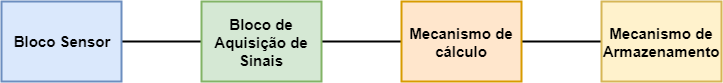
\includegraphics[width=0.85\columnwidth]{figuras/medidor_energia}
	\caption{Blocos funcionais de um medidor de energia.}
	\label{fig:medidor_energia}
\end{figure}

O Bloco Sensor � respons�vel por realizar as medi��es de forma anal�gica das grandezas de tens�o e corrente da rede el�trica, normalmente atrav�s de divisores de tens�o e por resistor \textit{shunt} - um resistor de baix�ssima resist�ncia - ou por um transformador de corrente, que induz uma tens�o a partir da corrente que passa por ele \cite{video_analog_devices}.
 
O Bloco de Aquisi��o de Sinais � encarregado de realizara a convers�o das grandezas de formato anal�gico para formato digital. Essa convers�o normalmente � feita a partir de conversores anal�gicos/digitais chamados de Delta-Sigma, de alta precis�o, por volta de 24 bits.

O Mecanismo de c�lculo computa os outros par�metros da rede el�trica, baseando-se nos valores de tens�o e corrente el�trica obtidos no Bloco Sensor, dessa forma consegue obter os valores de frequ�ncia, pot�ncia e fator de pot�ncia. Com isso, esses valores s�o ajustados para facilitar a interpreta��o. 

O Mecanismo de Armazenamento � incumbido de armazenar os dados fornecidos pelo Mecanismo de c�lculo em registrados para f�cil acesso. Estes registradores podem ser acessados de forma totalmente isolada por microcontroladores externos. Essa comunica��o � feita comumente por 2 protocolos principais I2C e SPI.

Conforme retratado pelo Bloco Sensor, existem duas formas de medir a corrente: Resistor de tipo \textit{shunt} ou transformador de corrente. O primeiro �  mais barato e apresenta uma linearidade maior em rela��o ao range de medi��o, por�m, quando o quesito � medi��o em altas correntes, o segunda leva vantagem, uma vez que a medi��o � do tipo indireta, ou seja, � mais seguro. 
 

%%%%%%%%%%%%%%%%%%%%%%%%%%%%%%%%%%%%%%%%%%%%%%
\chapter{Arquitetura}
\label{chapter:arquitetura}
%%%%%%%%%%%%%%%%%%%%%%%%%%%%%%%%%%%%%%%%%%%%%%

\begin{figure}[H]
	\centering
	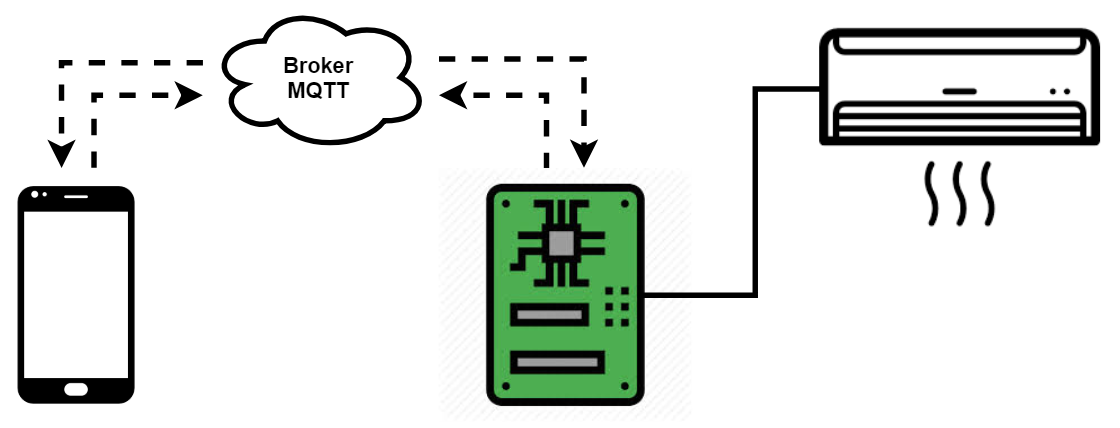
\includegraphics[width=0.8\columnwidth]{figuras/Architecture_Block_Diagram}
	\caption{Arquitetura a ser implementada.}
	\label{fig:Architecture_Block_Diagram}
\end{figure}

%%%%%%%%%%%%%%%%%%%%%%%%%%%%%%%%%%%%%%%%%%%%%%
\chapter{Desenvolvimento e Implementa��o}
\label{chapter:desenvolvimento}
Este cap�tulo apresenta detalhadamente o que foi feito para desenvolver e implementar o sistema de gerenciamento e controle de um condicionador de ar, levando em conta 3 pilares principais: \textit{Hardware}, \textit{Firmware} e \textit{Software}.
%%%%%%%%%%%%%%%%%%%%%%%%%%%%%%%%%%%%%%%%%%%%%%%%%%%%%%%%%%%%%%%%%%%%%%%%%%%%%%%%%%%%

%%%%%%%%%%%%%%%%%%%%%%%%%%%%%%%%%%%%%%%%%%%%%%%%%%%%%%%%%%%%%%%%%%%%%%%%%%%%%%%%%%%%
\section{\textit{Hardware}}
\label{section_hardware}
O desenvolvimento do \textit{hardware} iniciou-se com o levantamento dos circuitos el�tricos necess�rios para cumprir as fun��es requeridas conforme a concep��o do projeto, sendo eles: \textbf{Circuito de Conex�o com \textit{Wi-Fi}}, \textbf{Circuito de Ativa��o do Condicionador de Ar} e \textbf{Circuito de Sensoriamento}. O Circuito de Conex�o com \textit{Wi-Fi} �  respons�vel por trocar informa��es com o aplicativo mobile, utilizando o protocolo MQTT. O Circuito de Ativa��o do Condicionador de Ar � respons�vel  por permitir ou n�o a alimenta��o el�trica desse dispositivo. E o Circuito de Sensoriamento � respons�vel por realizar as medi��es provenientes da rede el�trica como tens�o, corrente, fator de pot�ncia e frequ�ncia com intuito de definir se os n�veis est�o adequados ao condicionador de ar e verificar a presen�a ou aus�ncia humana onde o equipamento est� instalado.

A elabora��o da PCB contendo os circuitos foi dividida em 4 partes principais: a escolha dos componentes a serem usados em cada circuito, o desenvolvimento dos esquem�ticos el�tricos, o desenvolvimento do \textit{layout} da placa de circuito impresso (PCB) e a prototipagem da PCB.
%%%%%%%%%%%%%%%%%%%%%%%%%%%%%%%%%%%%%%%%%%%%%%%%%%%%%%%%%%%%%%%%%%%%%%%%%%%%%%%%%%%%

%%%%%%%%%%%%%%%%%%%%%%%%%%%%%%%%%%%%%%%%%%%%%%%%%%%%%%%%%%%%%%%%%%%%%%%%%%%%%%%%%%%%
\subsection{Componentes utilizados} 
Para realizar a escolha dos componentes foi levado em conta principalmente o custo, visando tornar o produto atrativo ao usu�rio final, ou seja, o consumidor.

Para suprir as funcionalidades do \textbf{Circuito de Conex�o com \textit{Wi-Fi}}, o componente principal escolhido foi o m�dulo ESP12-F, representado na figura \ref{fig:ESP12-F}, que cont�m um microcontrolador juntamente com o circuito de radio-frequ�ncia (RF) para o \textit{Wi-Fi} e um LED indicativo. O microcontrolador contido no m�dulo � o ESP8266EX, representado na figura \ref{fig:ESP8266EX}, e suas principais caracter�sticas s�o\cite{ESP8266EX_DATASHEET}:

\begin{figure}[H]
	\centering
	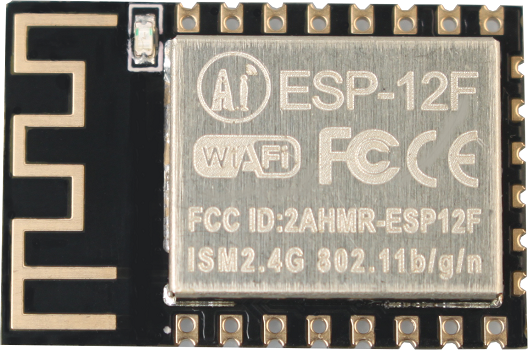
\includegraphics[width=0.4\columnwidth]{figuras/ESP12-F}
	\caption{M�dulo ESP12-F\cite{AiThinker}.}
	\label{fig:ESP12-F}
\end{figure}

\begin{figure}[H]
	\centering
	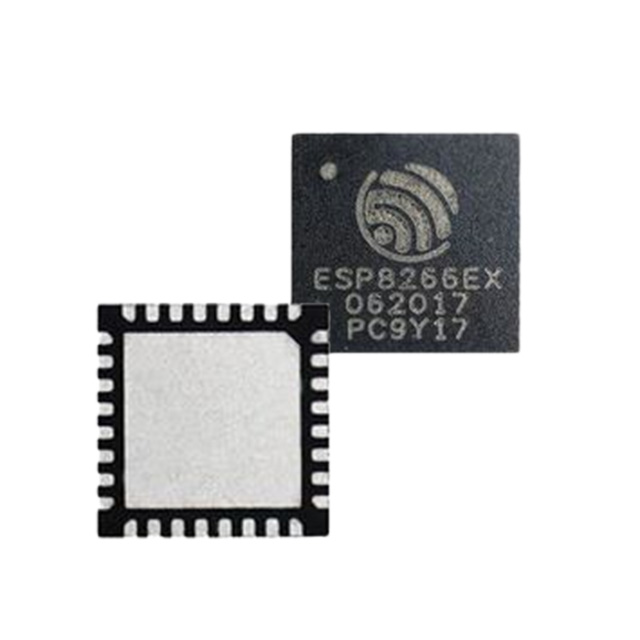
\includegraphics[width=0.4\columnwidth]{figuras/ESP8266EX}
	\caption{Microcontrolador ESP8266EX \cite{ESP8266_MICRO}.}
	\label{fig:ESP8266EX}
\end{figure}

\begin{itemize}
	\item Microprocessador de 32 bits;
	\item \textit{Wi-Fi} integrado sob o protocolo 802.11 b/g/n, na frequ�ncia de 2.4GHz;
	\item Interface perif�ricas: UART, SDIO, SPI, I2C, I2S, GPIO, ADC e PWM;
	\item Tens�o de opera��o: 2,5V a 3,6V;
	\item Corrente de opera��o: em m�dia 80mA;
	\item Tamanho: 5 mm x 5 mm;
	\item 32 pinos;
	\item Interface de grava��o tanto por UART, quanto por \textit{over-the-air} (OTA);
	\item At� 4 perfis de baixo consumo de energia.
\end{itemize}

Foram adicionados 2 (dois) \textit{light-emitting diodes} (LEDs) do tipo \textit{suface mounting device} (SMD), representado na figura \ref{fig:LED_SMD}, a este circuito tamb�m, um para indicar comunica��o com o celular pelo protocolo MQTT e um para indicar se a alimenta��o el�trica da PCB est� nos n�veis corretos, assim como 2 (dois) bot�es do tipo \textit{push-buttom}, representado na figura \ref{fig:Push_Button}, para realizar a grava��o do \textit{firmware} no microcontrolador.

\begin{figure}[H]
	\centering
	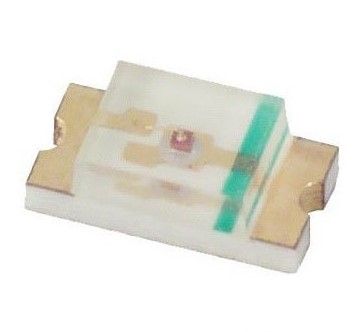
\includegraphics[width=0.4\columnwidth]{figuras/LED_SMD}
	\caption{LED SMD \cite{LED_SMD}.}
	\label{fig:LED_SMD}
\end{figure}

\begin{figure}[H]
	\centering
	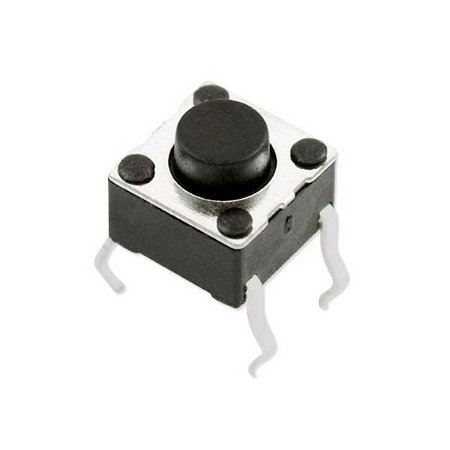
\includegraphics[width=0.4\columnwidth]{figuras/Push_Button}
	\caption{Bot�o do tipo \textit{push} \cite{Push_Button}.}
	\label{fig:Push_Button}
\end{figure}

Para o \textbf{Circuito de Ativa��o do Condicionador de Ar}, o principal componente escolhido foi o rel� SRD-05VDC-SL-C, representado na figura \ref{fig:srd-05vdc-sl-c}, quais caracter�sticas principais s�o:

\begin{itemize}
	\item Tens�o de ativa��o do enrolamento: 5 V;
	\item Corrente nominal do enrolamento: 89,3 mA;
	\item Resist�ncia do enrolamento: 55 $ \Omega $;
	\item Consumo de pot�ncia do enrolamento: 0,36 W;
	\item M�xima tens�o admiss�vel no chave: 110 VDC ou 225 VAC;
	\item Capacidade de corrente da chave para carga do tipo resistiva: 10 A para 125 VAC e 7 A para 240 VAC.
\end{itemize}

\begin{figure}[H]
	\centering
	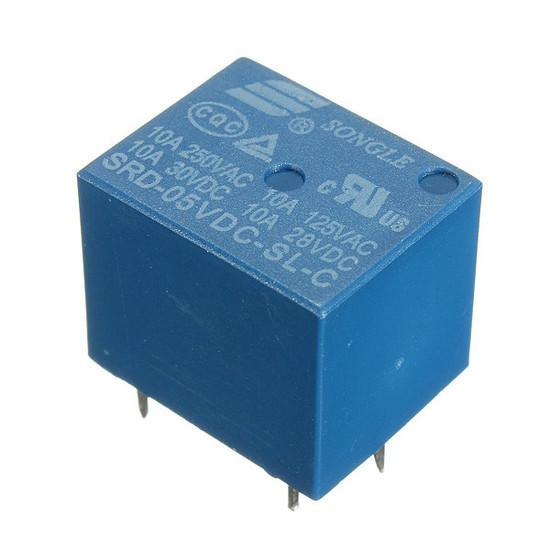
\includegraphics[width=0.4\columnwidth]{figuras/srd-05vdc-sl-c}
	\caption{Rel� SRD-05VDC-SL-C \cite{SRD-05VDC-SL-C_imagem}.}
	\label{fig:srd-05vdc-sl-c}
\end{figure}

O rel� SRD-05VDC-SL-C foi utilizado para ativar uma contatora que, por sua vez, alimenta o condicionador de ar. Como o objetivo foi de ativar qualquer tipo de condicionador de ar, utilizou-se contatoras, representadas na imagem \ref{fig:contatora}, que aceitassem tanto 110 VAC quanto 220 VAC no enrolamento de alimenta��o.

\begin{figure}[H]
	\centering
	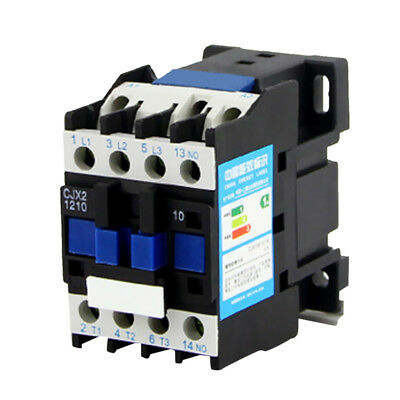
\includegraphics[width=0.4\columnwidth]{figuras/contatora}
	\caption{Contatora Telemecanique \cite{contatora_ref}.}
	\label{fig:contatora}
\end{figure}

Para o \textbf{Circuito de Sensoriamento}, o componente escolhido para fazer as medi��es de tens�o, corrente, fator de pot�ncia e frequ�ncia da rede de energia el�trica, informa��es essas suficientes para definir se ela est� adequada para alimentar o condicionador de ar, foi MCP39F521, representado na figura \ref{fig:MCP39F521}. O MCP39F521 � um dispositivo de monitoramento de energia monof�sico completo e altamente integrado, projetado para medi��o em tempo real de energia de entrada para fontes de alimenta��o de corrente alternada e de corrente cont�nua, unidades de distribui��o de energia, consumidor e aplica��es industriais. Inclui ADCs delta-sigma de canal duplo, um mecanismo de c�lculo de 16 bits, EEPROM e uma interface I2C de dois fios flex�vel. Uma refer�ncia integrada de tens�o de baixa deriva��o com 10 ppm/�C al�m de 94,5 dB de desempenho de sinal-ru�do e taxa de distor��o (SINAD) em cada canal de medi��o permite melhor que 0,1 $ \% $ de projetos precisos em uma faixa din�mica de 4000:1\cite{MCP39F521_Datasheet}. Foi adicionado tamb�m um sensor de temperatura anal�gico, por quest�es de seguran�a (superaquecimento), para monitorar a temperatura da PCB, MCP9700 que � representado pela figura \ref{fig:MCP9700}.

\begin{figure}[H]
	\centering
	
\includegraphics[width=0.4\columnwidth]{figuras/MCP39F521}
	\caption{Circuito Integrado (CI) MCP39F521 \cite{MCP39F521}.}
	\label{fig:MCP39F521}
\end{figure}

\begin{figure}[H]
	\centering
	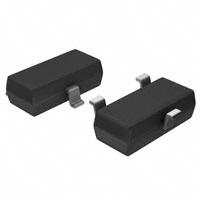
\includegraphics[width=0.4\columnwidth]{figuras/MCP9700}
	\caption{Circuito Integrado MCP9700 \cite{MCP9700}.}
	\label{fig:MCP9700}
\end{figure}
%%%%%%%%%%%%%%%%%%%%%%%%%%%%%%%%%%%%%%%%%%%%%%%%%%%%%%%%%%%%%%%%%%%%%%%%%%%%%%%%%%%%

%%%%%%%%%%%%%%%%%%%%%%%%%%%%%%%%%%%%%%%%%%%%%%%%%%%%%%%%%%%%%%%%%%%%%%%%%%%%%%%%%%%%
\subsection{Esquem�ticos el�tricos}
A partir dos circuitos el�tricos previamente citados, elaborou-se os esquem�ticos el�tricos baseando-se principalmente nos documentos de \textit{Reference Design} disponibilizados pelos fabricantes dos CI's utilizados. O documento principal utilizado foi o guia do usu�rio para o MCP39F521 \cite{MCP39f521_user_guide}, que auxiliou principalmente no \textbf{Circuito de Sensoriamento}.
%%%%%%%%%%%%%%%%%%%%%%%%%%%%%%%%%%%%%%%%%%%%%%%%%%%%%%%%%%%%%%%%%%%%%%%%%%%%%%%%%%%%

%%%%%%%%%%%%%%%%%%%%%%%%%%%%%%%%%%%%%%%%%%%%%%%%%%%%%%%%%%%%%%%%%%%%%%%%%%%%%%%%%%%%
\subsection{\textit{Layout} da PCB}
Para realizar o \textit{layout} da PCB, foi necess�rio levar em conta os pontos cr�ticos do circuito, que foram:

\begin{enumerate}
	\item[1.] Apresentar tens�o alternada de 110 ou 220 volts nominal, para alimenta��o do circuito mostrado nas Imagens \ref{fig:Schematic_Power_Supply}, \ref{fig:Schematic_Meter} e \ref{fig:Schematic_Core_Processor}, e os terminais de controle da contatora.
	\item[2.] Apresentar um LED 
\end{enumerate}

\subsection{Fabrica��o}


\subsection{M�dulo placa de automa��o de refrigera��o residencial}


\section{\textit{Firmware}}
\label{section_firmware}
Para elabora��o inicial do \textit{firmware}, foi utilizado o m�dulo NodeMCU Lol1n, mostrado na figura \ref{fig:nodemcu_lol1n}, que cont�m um m�dulo ESP-12E por�m com os circuitos de alimenta��o e grava��o por interface USB j� embutidos nele. Esta metodologia de utilizar um m�dulo pronto
foi utilizada com intuito de diminuir o tempo gasto com a elabora��o de um circuito para grava��o do microcontrolador e tamb�m para permitir o desenvolvimento do \textit{firmware} antes do t�rmino da fabrica��o, montagem dos componentes e testes el�tricos da PCB.

\begin{figure}[H]
	\centering
	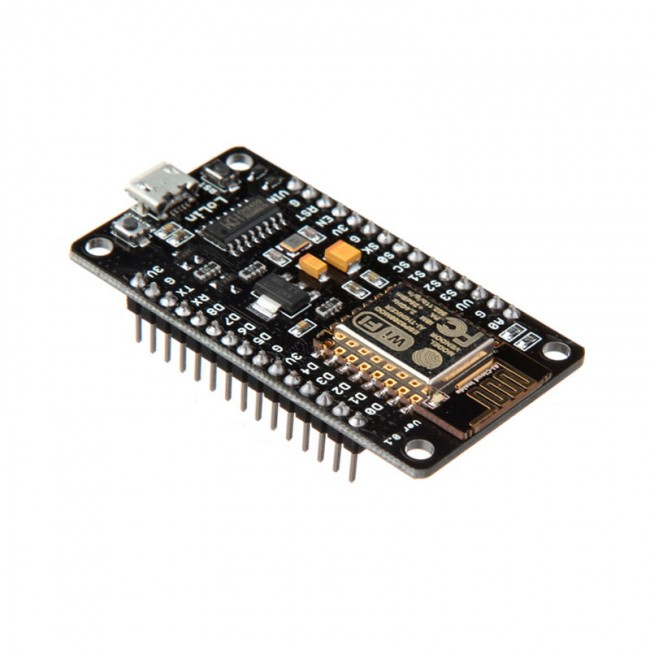
\includegraphics[width=0.4\columnwidth]{figuras/nodemcu_lol1n}
	\caption{M�dulo NodeMCU Lol1n.}
	\label{fig:nodemcu_lol1n}
\end{figure}

\subsection{Comunica��o no protocolo MQTT}

\subsection{Monitoramento de presen�a humana}

\subsection{Monitoramento da qualidade da energia el�trica}



\section{\textit{Software}}
\label{section_software}

\subsection{Comunica��o no protocolo MQTT}

\subsection{Intera��o com o \textit{Hardware} implementado}

\subsection{Funcionalidades implementadas}





%%%%%%%%%%%%%%%%%%%%%%%%%%%%%%%%%%%%%%%%%%%%%%
\chapter{Testes e Avalia��o de Desempenho}
\label{chapter:chapter_testes_avaliacao}
%%%%%%%%%%%%%%%%%%%%%%%%%%%%%%%%%%%%%%%%%%%%%%

Para a realiza��o dos testes

\begin{figure}[H]
	\centering
	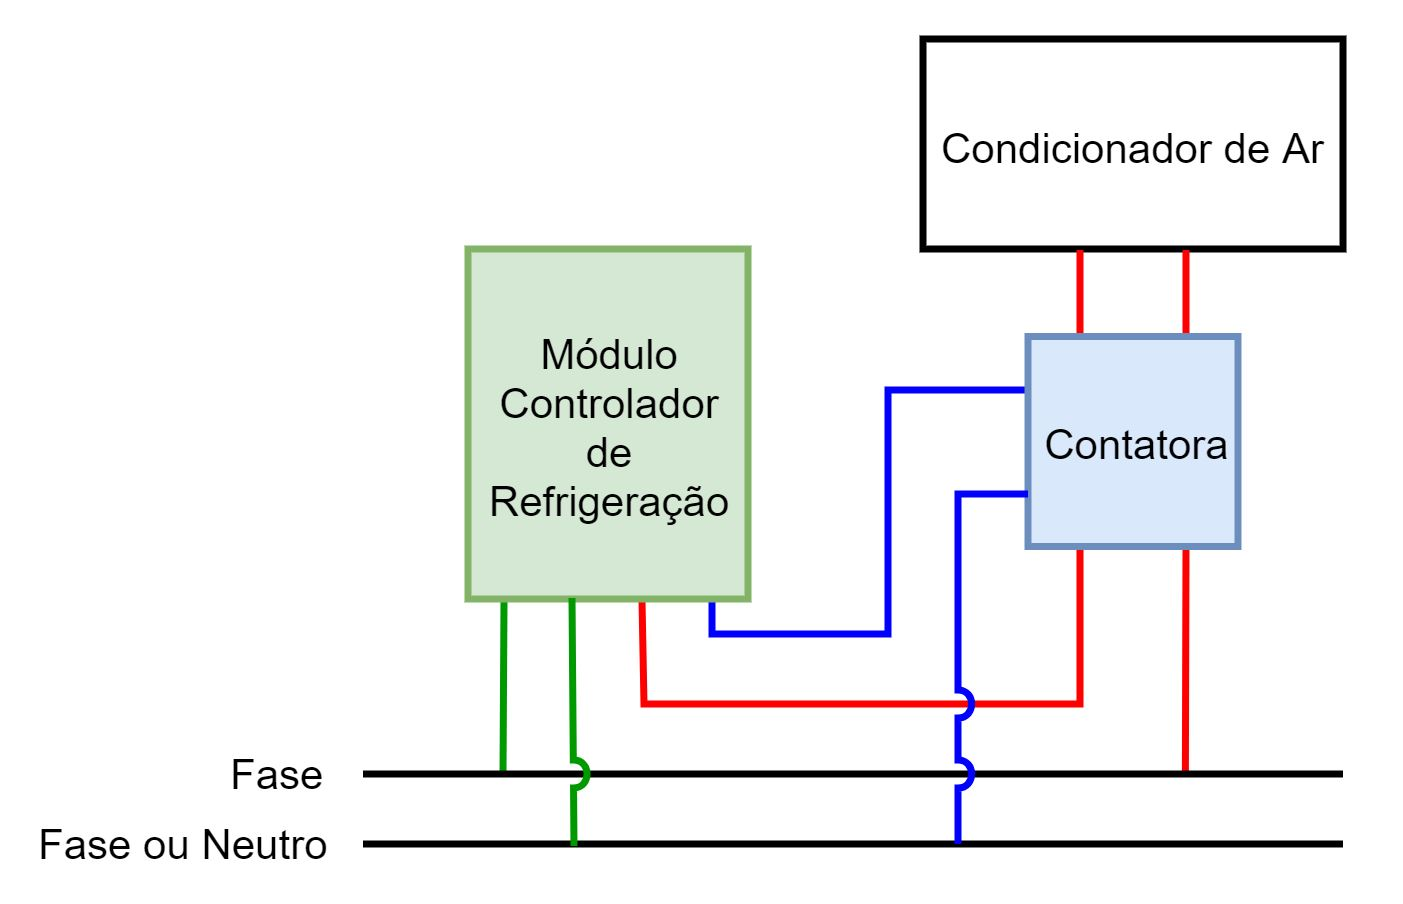
\includegraphics[width=0.8\columnwidth]{figuras/hardware_connection_diagram}
	\caption{Diagrama de conex�o do hardware.}
	\label{fig:hardware_connection_diagram}
\end{figure}

\begin{figure}[H]
	\centering
	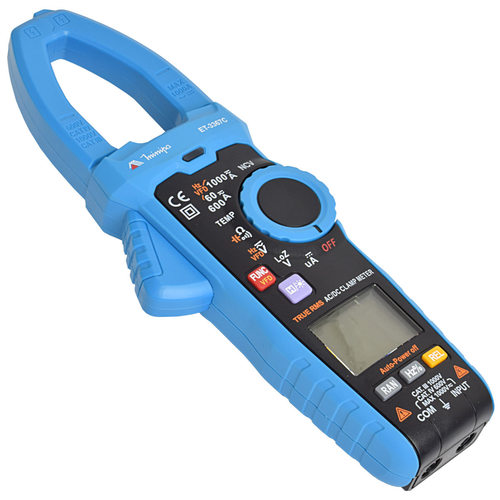
\includegraphics[width=0.4\columnwidth]{figuras/alicate_amperimetro_minipa}
	\caption{Alicate amper�metro ET-3367C \cite{alicate_amperimetro_minipa}.}
	\label{fig:alicate_amperimetro_minipa}
\end{figure}

\begin{table}[h!]
	\caption{Medi��o da corrente alternada}	
	\label{table:medicao_corrente}
	\begin{tabular}{|c|c|}
		\hline
		 Medidas de corrente pela placa [A] & Medidas de corrente pelo alicate amper�metro [A] \\ \hline
		4.21 & 4.2 \\ \hline
		4.27 & 4.32 \\ \hline
		4.45 & 4.46 \\ \hline
		4.49 & 4.51 \\ \hline
		4.6 & 4.6 \\ \hline
		4.6 & 4.61 \\ \hline
		4.63 & 4.63 \\ \hline
		4.66 & 4.67 \\ \hline
		4.71 & 4.71 \\ \hline
		4.73 & 4.73 \\ \hline
		4.78 & 4.77 \\ \hline
		4.81 & 4.8 \\ \hline
		4.84 & 4.86 \\ \hline
		4.88 & 4.89 \\ \hline
		4.89 & 4.9 \\ \hline
		4.93 & 4.93 \\ \hline
		4.95 & 4.96 \\ \hline
		4.96 & 5 \\ \hline
		5.03 & 5.04 \\ \hline
		5.04 & 5.04 \\ \hline
		5.07 & 5.1 \\ \hline
		5.1 & 5.11 \\ \hline
		5.15 & 5.14 \\ \hline
		5.11 & 5.14 \\ \hline
		5.14 & 5.14 \\ \hline
		5.16 & 5.17 \\ \hline
		5.16 & 5.18 \\ \hline
		5.19 & 5.19 \\ \hline
		5.25 & 5.25 \\ \hline
		5.26 & 5.27 \\ \hline	
	\end{tabular}
\end{table}

\begin{table}[h!]
	\caption{Medi��o da tens�o alternada}	
	\label{table:medicao_tensao}
	\begin{tabular}{|c|c|}
		\hline
		Medidas de tens�o pela placa [V] & Medidas de tens�o pelo alicate amper�metro [V] \\ \hline
		221.8 & 222.8 \\ \hline
		221.6 & 222.3 \\ \hline
		221.6 & 222.4 \\ \hline
		222.8 & 223.1 \\ \hline
		222.5 & 223.5 \\ \hline
		222 & 223.6 \\ \hline
		222.4 & 223.6 \\ \hline
		222.3 & 223.5 \\ \hline
		221.3 & 223.2 \\ \hline
		221.6 & 222.5 \\ \hline
		221.4 & 222.6 \\ \hline
		221.3 & 222.2 \\ \hline
		222.1 & 222.3 \\ \hline
		222 & 223 \\ \hline
		222.3 & 222.9 \\ \hline
		221.9 & 223.1 \\ \hline
		222 & 223 \\ \hline
		222.3 & 223.1 \\ \hline
		221.5 & 222.7 \\ \hline
		221.2 & 222.6 \\ \hline
		221.5 & 222.7 \\ \hline
		221.3 & 222.4 \\ \hline
		221.6 & 222.7 \\ \hline
		221.6 & 222.6 \\ \hline
		222.3 & 223.3 \\ \hline
		222.3 & 223.3 \\ \hline
		222.1 & 223.4 \\ \hline
		222.2 & 223.5 \\ \hline
		221.5 & 223.4 \\ \hline
		221.8 & 222.8 \\ \hline
	\end{tabular}
\end{table}

\begin{table}[h!]
	\caption{Medi��o da frequ�ncia}	
	\label{table:medicao_frequencia}
	\begin{tabular}{|c|c|}
		\hline
		Medidas de frequ�ncia pela placa [V] & Medidas de frequ�ncia pelo alicate amper�metro [V] \\ \hline
		59.91 & 60.03 \\ \hline
		59.94 & 60.06 \\ \hline
		59.89 & 60.01 \\ \hline
		59.89 & 60.02 \\ \hline
		59.89 & 60.02 \\ \hline
		59.94 & 59.99 \\ \hline
		59.91 & 60 \\ \hline
		59.91 & 59.98 \\ \hline
		59.94 & 60.02 \\ \hline
		59.89 & 60.04 \\ \hline
		59.89 & 59.99 \\ \hline
		59.94 & 59.98 \\ \hline
		59.89 & 60 \\ \hline
		59.94 & 60.01 \\ \hline
		59.89 & 60.02 \\ \hline
		59.84 & 59.95 \\ \hline
		59.96 & 60.02 \\ \hline
		59.86 & 59.98 \\ \hline
		59.86 & 59.98 \\ \hline
		59.94 & 60.03 \\ \hline
		59.89 & 59.99 \\ \hline
		59.91 & 59.97 \\ \hline
		59.91 & 59.99 \\ \hline
		59.91 & 60.01 \\ \hline
		59.94 & 60.01 \\ \hline
		59.99 & 60.02 \\ \hline
		59.94 & 60.03 \\ \hline
		59.89 & 60 \\ \hline
		59.94 & 59.98 \\ \hline
		59.89 & 59.99 \\ \hline
	\end{tabular}
\end{table}
\input{6_Conclusao/Conclusao}

\appendix
%%%%%%%%%%%%%%%%%%%%%%%%%%%%%%%%%%%%%%%%%%%%%%
\chapter{Esquem�ticos El�tricos}
\label{chapter:apendice_a}
%%%%%%%%%%%%%%%%%%%%%%%%%%%%%%%%%%%%%%%%%%%%
\begin{figure}[H]
	\centering
	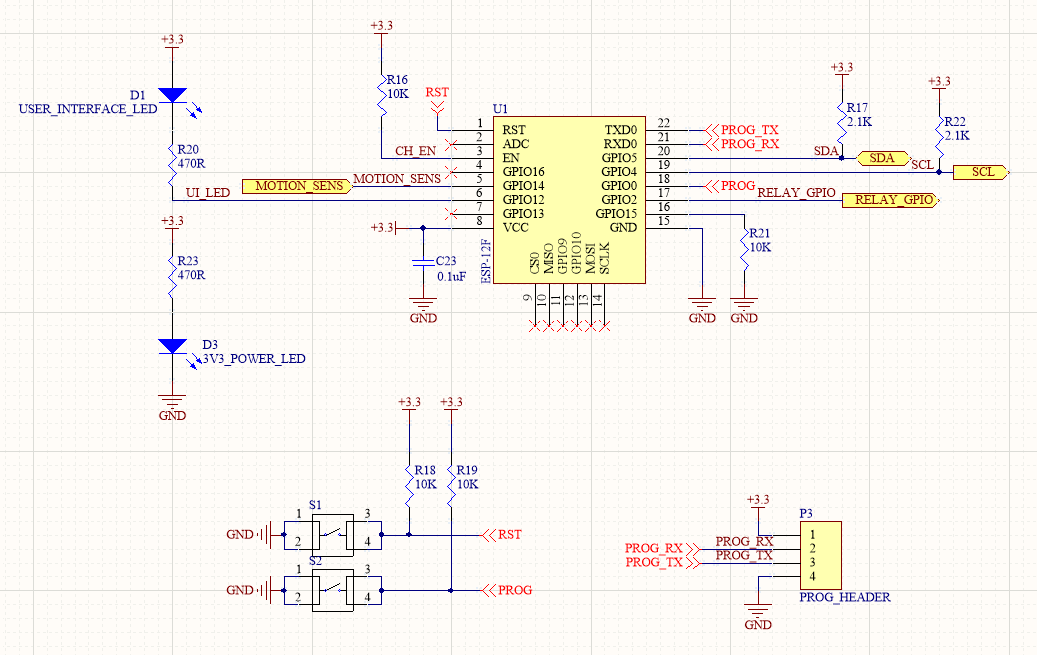
\includegraphics[angle = 90, width=0.65\columnwidth]{figuras/Schematic_Core_Processor}
	\caption{Esquem�tico el�trico referente ao microcontrolador.}
	\label{fig:Schematic_Core_Processor}
\end{figure}

\begin{figure}[H]
	\centering
	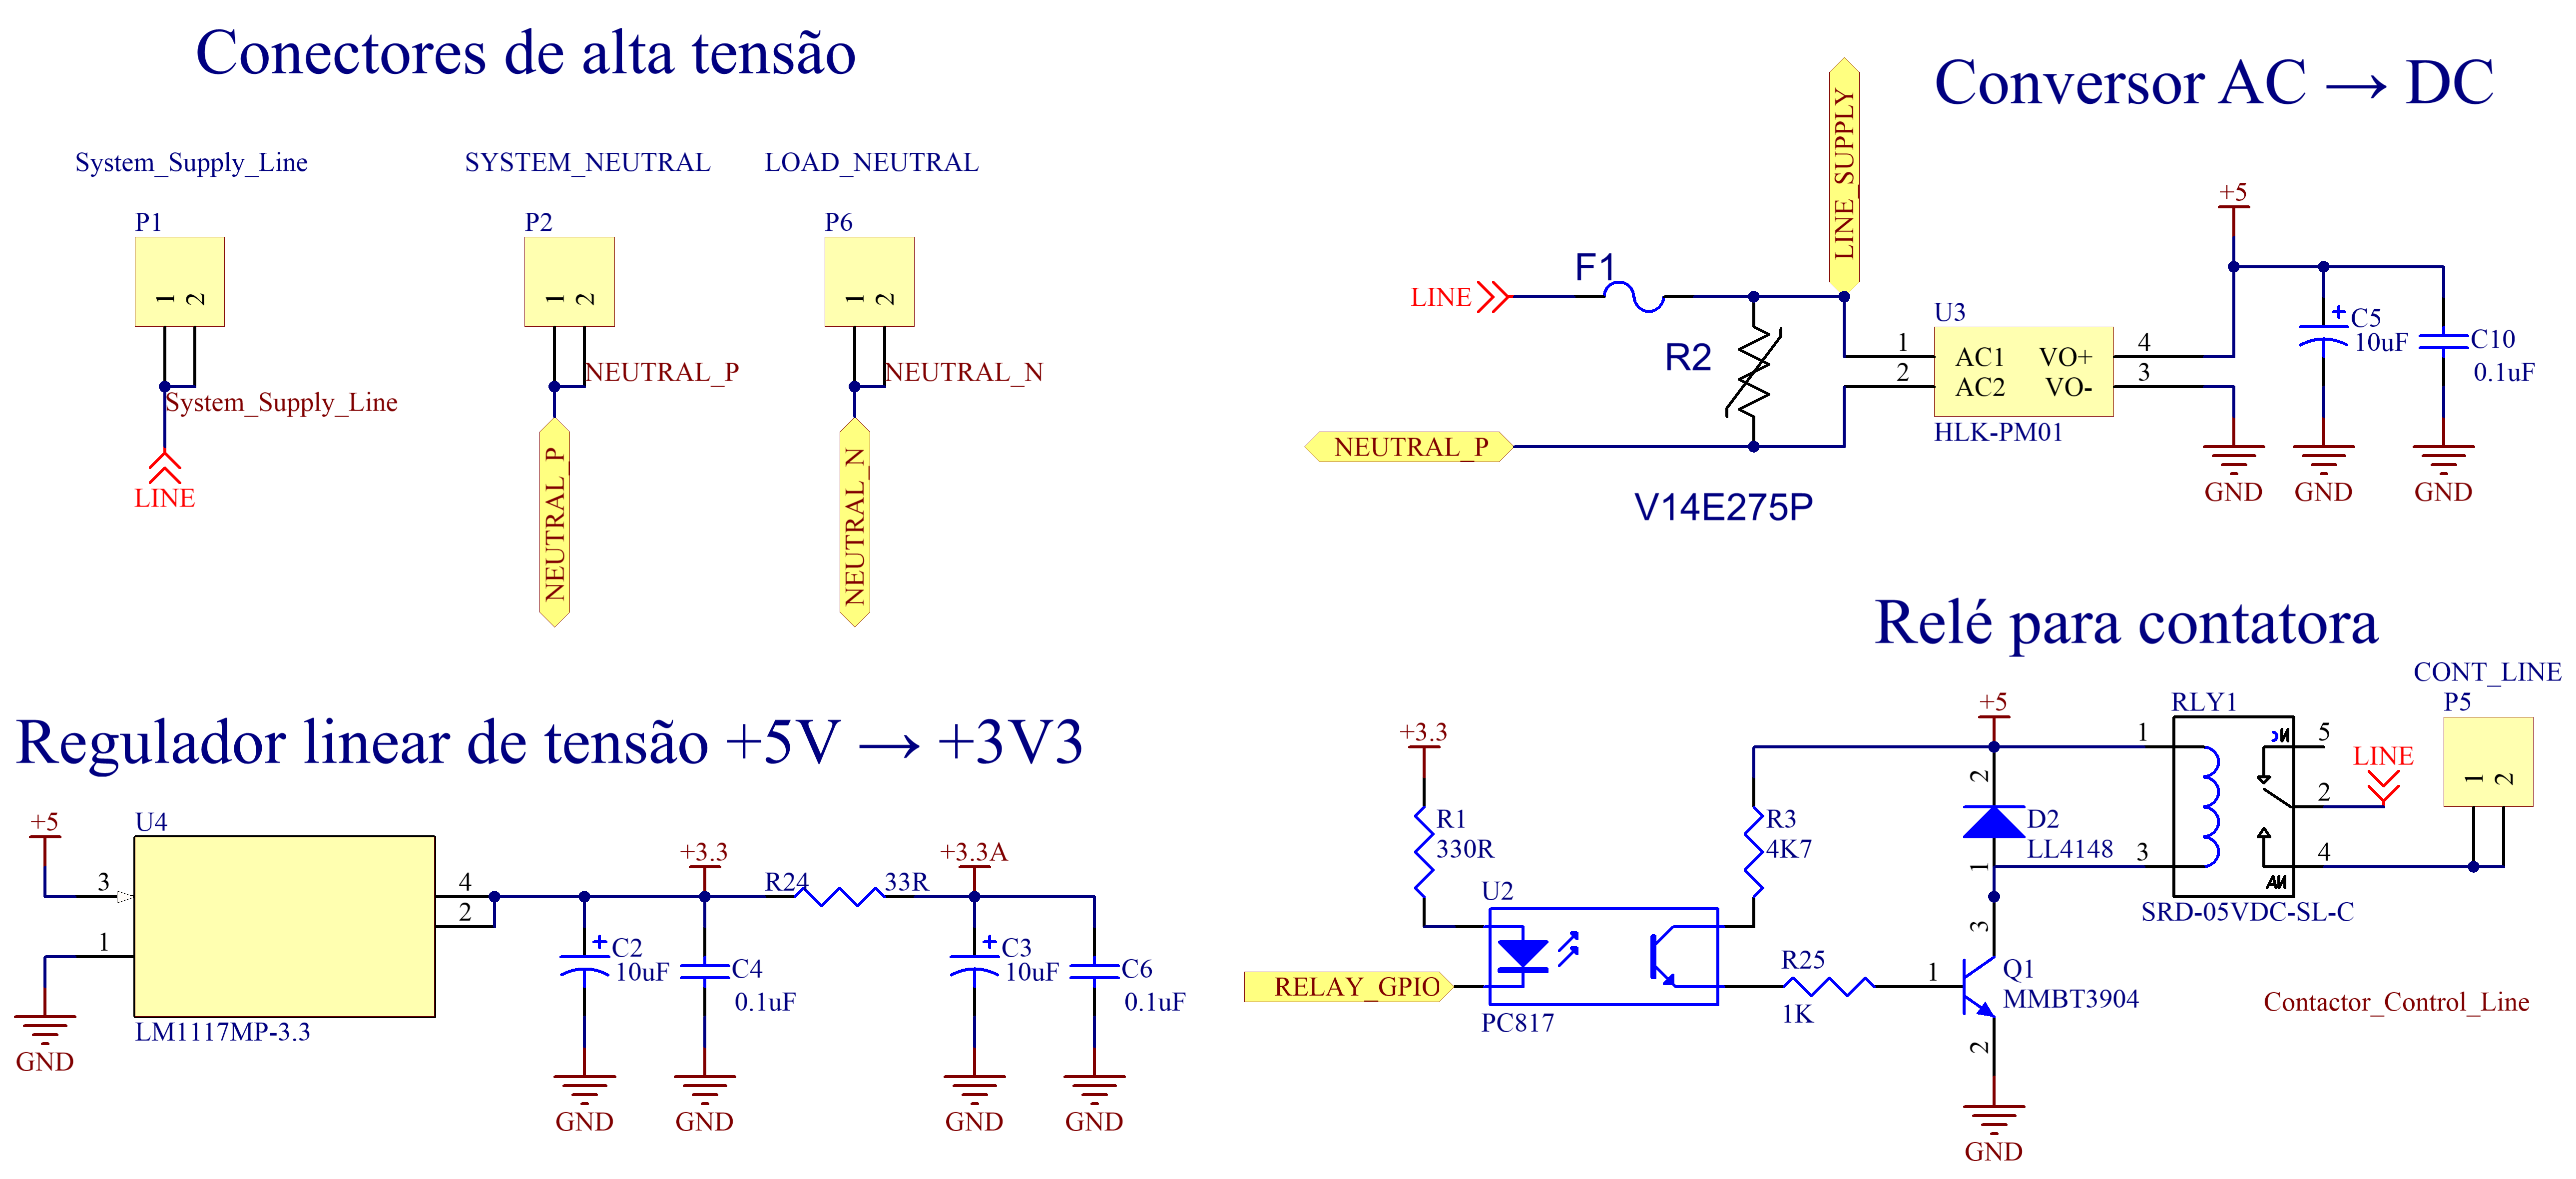
\includegraphics[angle = 90, width=0.8\columnwidth]{figuras/Schematic_Power_Supply}
	\caption{Esquem�tico el�trico da alimenta��o do circuito.}
	\label{fig:Schematic_Power_Supply}
\end{figure}

\begin{figure}[H]
	\centering
	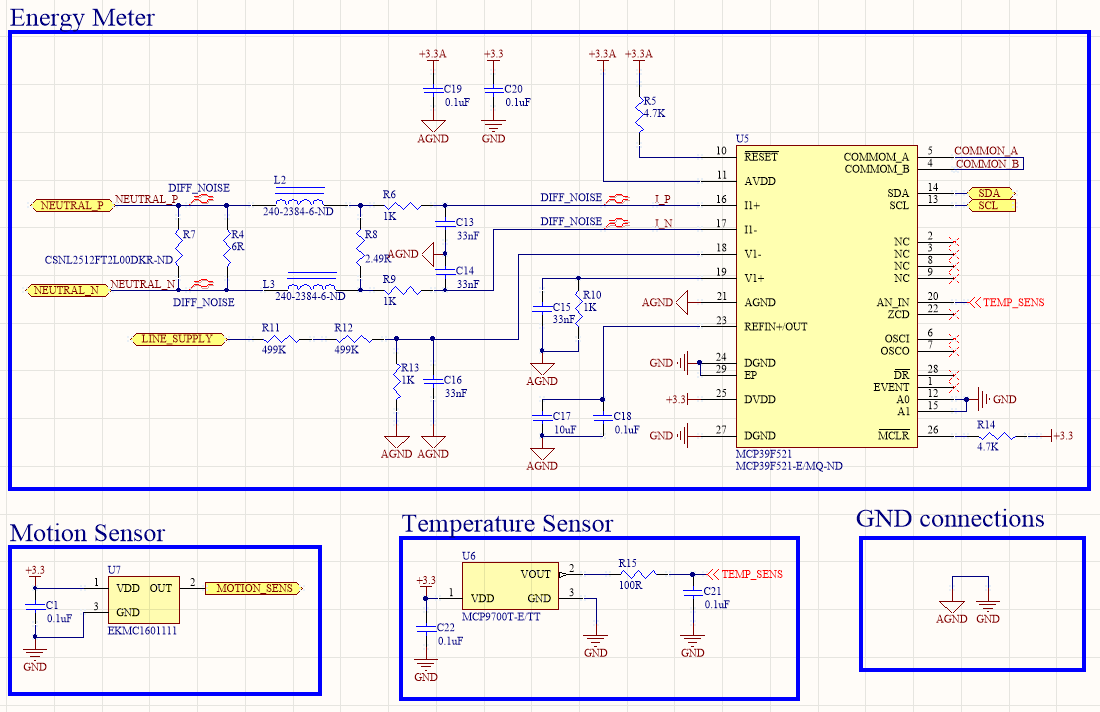
\includegraphics[angle = 90, width=0.9\columnwidth]{figuras/Schematic_Meter}
	\caption{Esquem�tico el�trico do sistema de medi��o da energia el�trica.}
	\label{fig:Schematic_Meter}
\end{figure}

\chapter{\textit{Layout} da PCB}
\label{chapter:apendice_b}
\begin{figure}[H]
	\centering
	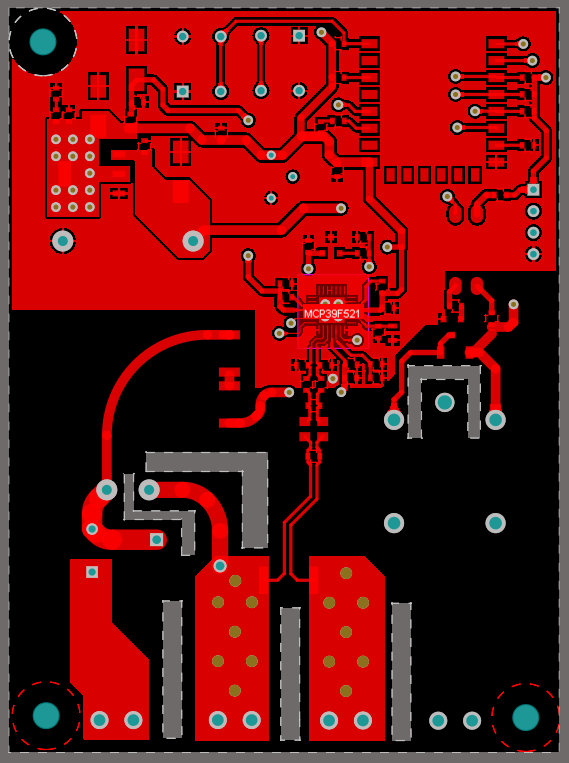
\includegraphics[width=0.8\columnwidth]{figuras/Layout_Top}
	\caption{\textit{Top Layer} do \textit{layout} da PCB.}
	\label{fig:Layout_Top}
\end{figure}

\begin{figure}[H]
	\centering
	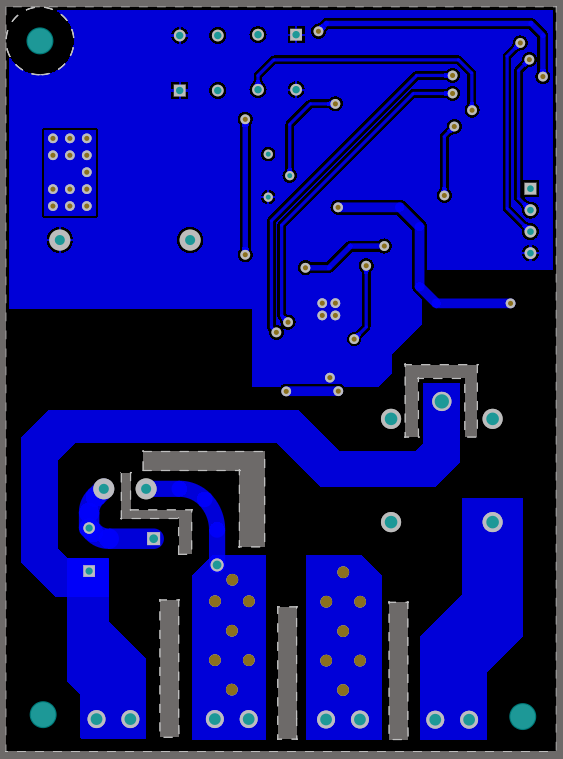
\includegraphics[width=1\columnwidth]{figuras/Layout_Bottom}
	\caption{\textit{Bottom Layer} do \textit{layout} da PCB.}
	\label{fig:Layout_Bottom}
\end{figure}

\begin{figure}[H]
	\centering
	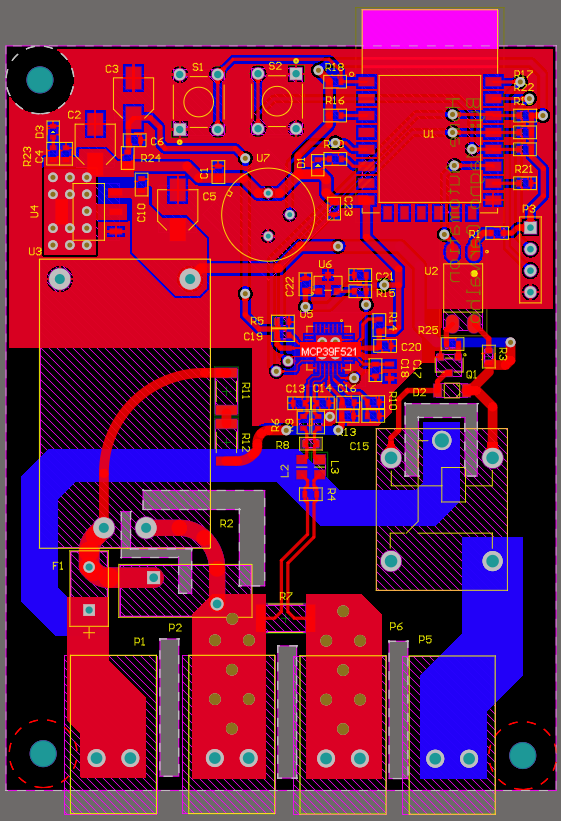
\includegraphics[width=1\columnwidth]{figuras/Layout_All_Layers}
	\caption{\textit{Layout} da PCB contendo os \textit{Layers Top} e \textit{Bottom}, os componentes e suas serigrafias.}
	\label{fig:Layout_All_Layers}
\end{figure}

\begin{figure}[H]
	\centering
	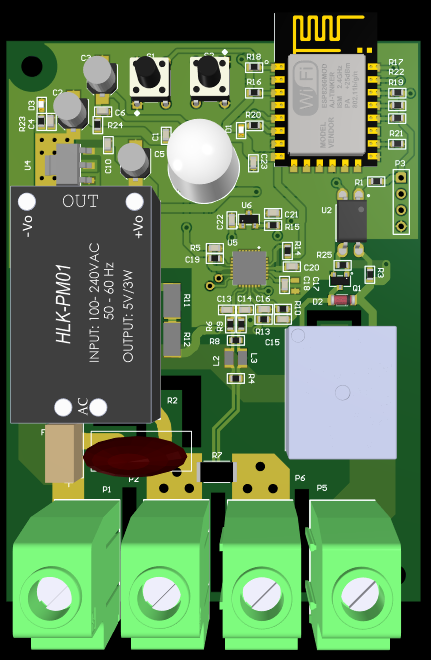
\includegraphics[width=1\columnwidth]{figuras/Layout_3D_Top}
	\caption{Vis�o superior da representa��o 3D do \textit{layout} da PCB.}
	\label{fig:Layout_3D_Top}
\end{figure}

\begin{figure}[H]
	\centering
	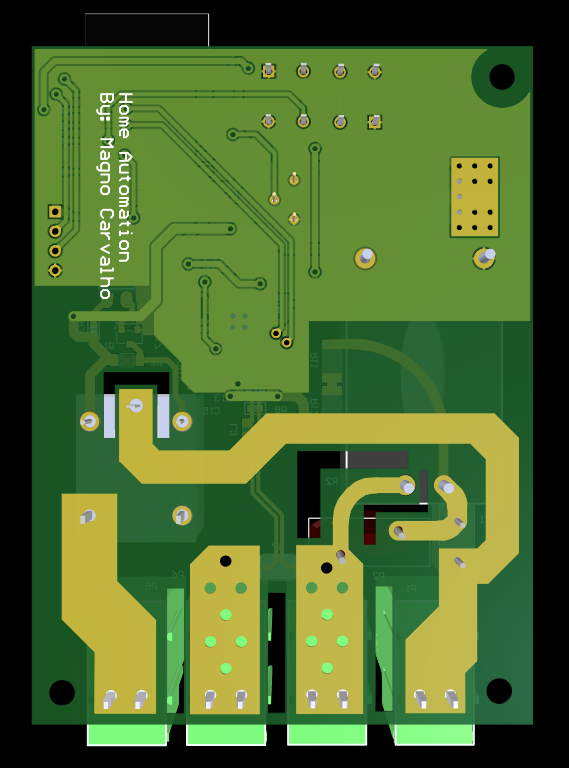
\includegraphics[width=1\columnwidth]{figuras/Layout_3D_Bottom}
	\caption{Vis�o inferior da representa��o 3D do \textit{layout} da PCB.}
	\label{fig:Layout_3D_Bottom}
\end{figure}

\begin{figure}[H]
	\centering
	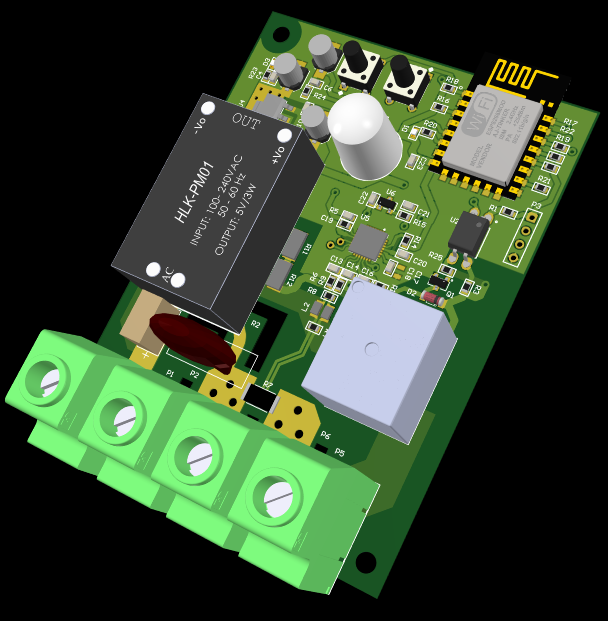
\includegraphics[width=1\columnwidth]{figuras/Layout_3D_Isometric}
	\caption{Vis�o isom�trica da representa��o 3D do \textit{layout} da PCB.}
	\label{fig:Layout_3D_Isometric}
\end{figure}



\cleardoublepage
\pagestyle{bibliography}
\bibliographystyle{abntex2-num}
%\bibliographystyle{IEEEtran}
\bibliography{bibliografia/refs}

\end{document}